\documentclass[final, ms, a4paper, 11pt]{memoir}

\usepackage[a4paper, inner=3cm, outer=3cm, marginpar=0pt]{geometry}
\usepackage[explicit]{titlesec}
\usepackage{csvsimple}
\usepackage{wrapfig}
\usepackage{graphicx}
\usepackage{xcolor} %

% set line height
\renewcommand{\baselinestretch}{1}
% font hyphenation
\usepackage{everysel}
\EverySelectfont{%
\fontdimen2\font=0.6em % interword space
\fontdimen3\font=0.2em % interword stretch
\fontdimen4\font=0.1em % interword shrink
\fontdimen7\font=0.9em % extra space
\hyphenchar\font=`\-% to allow hyphenation
}


% set section style
% \newcommand{\secstyle}[2]{[ #2 ] \textcolor{red!50!black}{\MakeUppercase{#1}}}
% \renewcommand*\thesection{\arabic{section}} % hide chapter

\newcommand\ddate{01.01.1970}
\titleformat{\section}
  {\normalfont}{- \ddate{}:}{1em}
  {\textcolor{red!50!black}{\MakeUppercase{#1}} -}
% monochrome
% \titleformat{\section}
%   {\normalfont}{\thesection}{1em}{\MakeUppercase{#1}}

\begin{document}
\noindent {\Large Z80 Single Board Computer: Note e Diario di Lavoro} \\\\
\noindent SAM Bellinzona 2016/2017 \\
\noindent REF: Daniele Kamm \\
\noindent PIF: Naoki Pross \\
\vspace{5mm}

\renewcommand\ddate{30.01.2017}
\section{Perch\`e uno Z80?}
Originariamente questo progetto era un esperimento per costruire una
cartridge per il GameBoy Classic (DMZ-01) che conteneva dell'hardware
aggiuntivo che avrebbe potuto interfacciare dell'hardware esterno con la CPU
del GameBoy. Successivamente per\`o il progetto si \`e rivelato pi\`u
complicato del previsto a causa della complessa struttura del GB (GameBoy) e
la difficolt\`a per ritrovare l'hardware stesso. Quindi sotto consiglio del
docente ho cambiato il progetto in un Single Board Computer dato che sono
interessato in informatica di basso livello e la CPU del GB era basata sul
processore Z80 con un instruction set e assembly simile.

\renewcommand\ddate{09.02.2017}
\section{Hardware}
Dopo una ricerca abbastanza intensiva dal magazzino della scuola abbiamo trovato
i seguenti componenti principali del che utilizzer\`o per costruire il computer.
\begin{table}[h!] \centering
\begin{tabular}{ l l l l }
    Z8400AB1 (Z80ACPU) & Zilog   & x1 & CPU \\
    Z8420AB1 (Z80APIO) & Zilog   & x1 & Port Interface \\
    Z8430AB1 (Z80ACTC) & Zilog   & x1 & Timer Clock \\
    M28C64             & ST      & x2 & EEPROM \\
    HM62256B           & HITACHI & x1 & SRAM \\
    TL16C550C          & TI      & x1 & Seriale (UART / RS232) \\
\end{tabular}
\end{table}

Tutti gli altri componenti secondati come porte logiche e circuiti combinatori
integrati saranno indicati in una lista finale nella documentazione riassuntiva.

\renewcommand\ddate{13.02.2017}
\section{Address space}
% \begin{wrapfigure}{R}{.35\linewidth} \centering
%     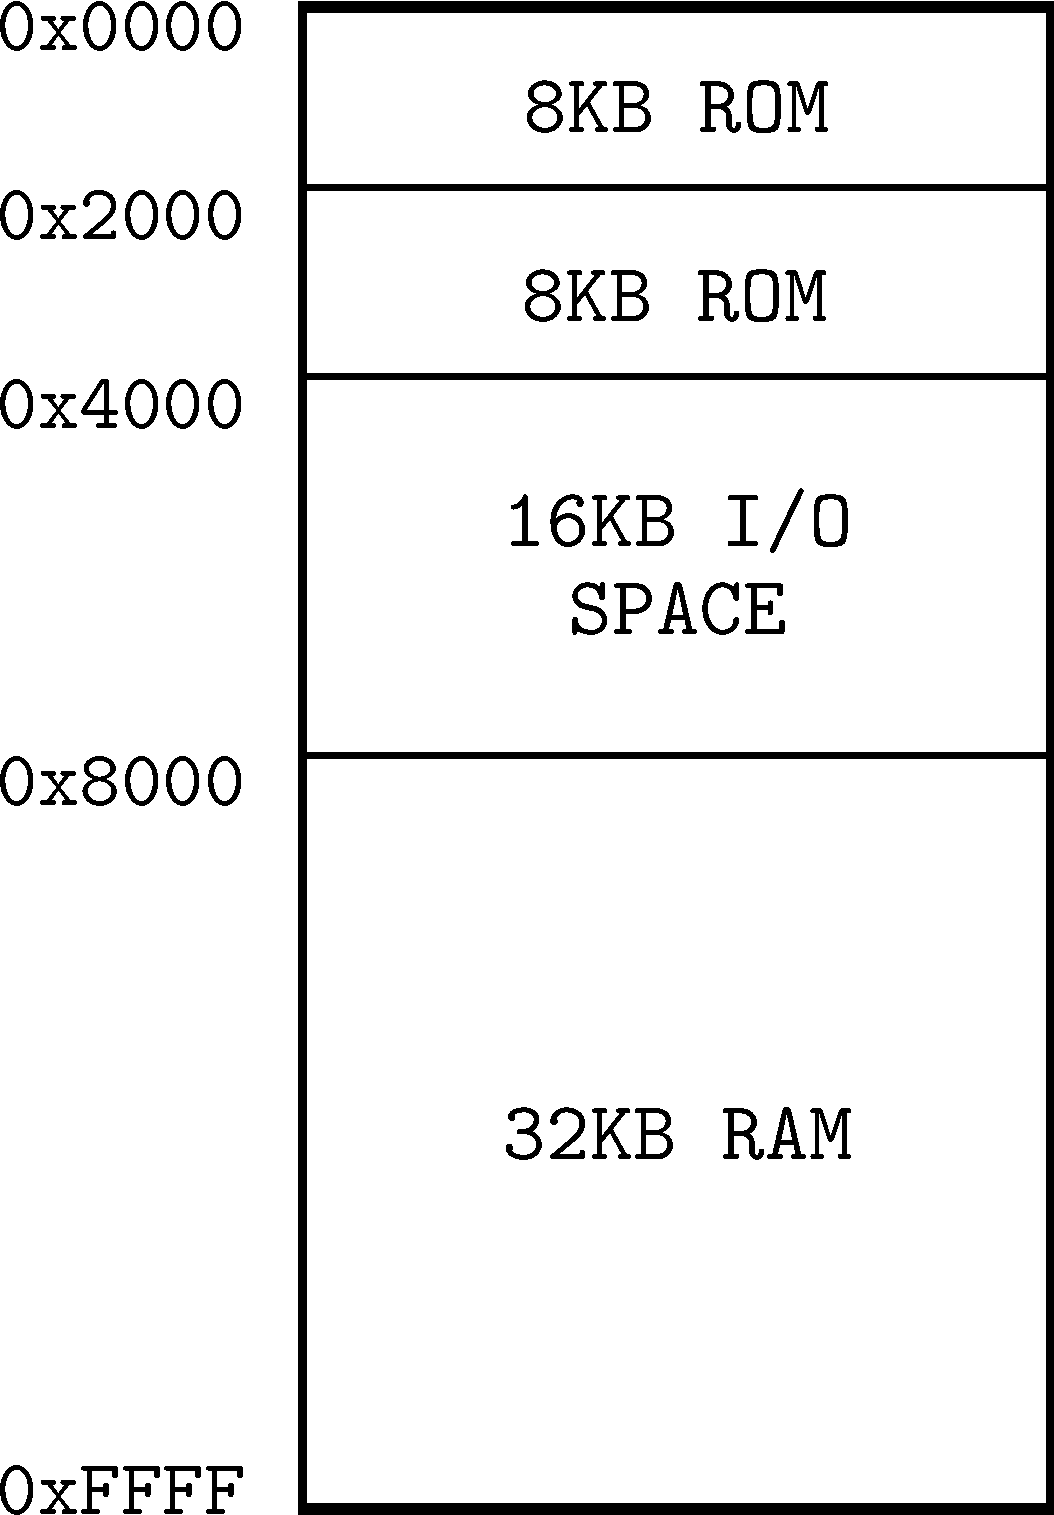
\includegraphics[width=.9\linewidth]{res/addrspace.pdf}
% \end{wrapfigure}
Come prima cosa dopo aver deciso il processore (Z80) \`e necessario definire
l'address space per decidere come collegare l'hardware. Si vede chiaramente che
la RAM usa la maggior parte dell'address space mentre la rom \`e solamente di
16KB, ma questo non \`e un problema perch\`e ho intenzione di aggiungere delle
interfacce esterne per poter collegare dispositivi di memoria come per esempio
le uSD. Dunque questa EEPROM vicina al processore sar\`a utilizzata unicamente
per il bootloader e per un sistema operativo molto basilare.

% \renewcommand\ddate{23.02.2017}
% \section{Banchi di memoria e paging della RAM}

\renewcommand\ddate{06.03.2017}
\section{Schede normate e clock secondari}
In seguito ad una discussione ho deciso di implementare il circuito su un PCB di
dimensioni standard, come per esempio l'Eurocard (IEEE 1101.10) in maniera da
poter montare tutte le schede su un rack. Cos\`i facendo si avrebbe dei
connettori standard sul retro che si potrebbero utilizzare per le periferiche
esterne. Alternativamente si potrebbe utilizzare una struttura simile al PC/104
permettendo di interfacciare delle periferiche specifiche per computer ancora
diponibili sul mercato. Il connettore standard per PC/104 \`e un header 32x2,
quindi con 64 pin mappato come indicato sotto, con un opzionale estensione che
pu\`o aumentare il connettore a 146
pins\footnote{http://pinouts.ru/Slots/Pc104\_pinout.shtml}.

\csvautotabular{res/pc104conn.csv}

\renewcommand\ddate{07.03.2017}
\section{Tastiera Misteriosa}
Nello stesso luogo in cui avevo trovato lo Z80 stesso ho trovato anche una
tastiera con un connettore mai visto. Il connettore era composto da 19 pin, di
cui 16 erano collegati all'interno della tastiera. Inizialmente pensavo che la
tastiera contenesse gi\`a un driver che generava degli interrupt, come una
qualsiasi tastiera moderna, con l'unica differenza che il bus di comunicazione
era parallelo. Ma dopo una ricerca rapida senza risultati ho deciso di aprire la
tastiera per analizzare il layout. Inaspettatamente ho scoperto che l'intero PCB
non \`e altro che una griglia 9x9 con i 18 fili che portano al connettore.
Questo hardware probabilmente era per un C64 Commodore 64 che aveva il resto
della logica programmata nella ROM o sulla scheda madre.

Per utilizzare l'hardware in questo stato \`e dunque necessario attivare i
primi 9 bit del connettore e successivamente leggere i seguenti 9 mascherando il
tasto interessato. Qui sotto ho preso un esempio che ho trovato online per
dimostrare il concetto in assembly.

\begin{centering}
\begin{verbatim}
; This program waits until the key "S" was pushed.
; Start with SYS 49152

*=$c000                  ; startaddress 

PRA  =  $dc00            ; CIA#1 (Port Register A)
DDRA =  $dc02            ; CIA#1 (Data Direction Register A)

PRB  =  $dc01            ; CIA#1 (Port Register B)
DDRB =  $dc03            ; CIA#1 (Data Direction Register B)


start    sei             ; interrupts deactivated

         lda #%11111111  ; CIA#1 port A = outputs 
         sta DDRA             

         lda #%00000000  ; CIA#1 port B = inputs
         sta DDRB             

         lda #%11111101  ; testing column 1 (COL1) of the matrix
         sta PRA
            
loop     lda PRB
         and #%00100000  ; masking row 5 (ROW5) 
         bne loop        ; wait until key "S" 

         cli             ; interrupts activated

ende     rts             ; back to BASIC
\end{verbatim}
\end{centering}

\renewcommand\ddate{16.03.2017}
\section{Visualizzare e i dati}
Avendo messo un ``clock-stepper'' probabilmente \`e utile poter anche
visualizzare i valori esadecimali sul bus di dati e di indirizzi, dunque ho
pensato di aggiungere dei display a 7 segmenti collegati alle 8 e 16 linee dei
due bus, 

\end{document}
